\documentclass[11pt]{article}
\usepackage{colacl}
\usepackage{multirow}
\usepackage{graphicx}
\usepackage{helvet}  %Required
\usepackage{courier}  %Required
\usepackage{url}  %Required
\usepackage{subfigure}
\usepackage{algorithm}
\usepackage{algorithmic}
\usepackage{amsmath} 
\usepackage{xcolor}
\sloppy



\title{COMP90049 Knowledge Technologies \\
	Project 2: Which emoji is missing?}
%\author
%{Haonan Li \\
%haonanl5@student.unimelb.edu.au}



\begin{document}
\maketitle

\section{Introduction}

Emojis are ideograms which are naturally combined with plain text to visually complement or condense the meaning of a message. Plenty of researches on Emoji emerge in recent years, especially in Natural Language Processing area.

\cite{Aoki2011A} propose a method to create emotional vectors of emoticons automatically, \cite{Cappallo:2015:IZE:2733373.2806335} presents a model that can generating emoji labels for an image in a zero-shot manner. \cite{Barbieri2016What} analyze emojis used in Twitter and \cite{Barbieri2017Are} investigate the relation between words and emojis, studying the novel task of predicting which emojis are evoked by text-based tweet messages. Which is similar with our work. 

In this work, we employ two classification frameworks Naive Bayes and Decision Tree, to automatically predict the missing emoji of a Twitter message. We build two classifiers and apply them to the same dataset. The evaluations are based on precision, recall and F1-score.

\section{Dataset and Task}

\noindent\textbf{Dataset:} We sent rate-limited queries and retrieved tweets through the Twitter API\footnote{https://developer.twitter.com/en/docs/tweets/search/api-reference/ get-search-tweets} over several days in April 2018. These queries consisted of one of the 10 widely used emojis. To make the returned result suitable for classification task, we remove tweets containing two or more of the queried emojis and tweets not containing the emoji in the visible text. The remaining tweets are shuffled, and randomly assigned to training, development and test sets.

\noindent\textbf{Task:} We remove the emoji from the queried tweets and use it as a label for training and testing. The task for our machine learning models is to predict the single emoji that appears in the input tweet.

\section{Model}

There are two models in our project, Naive Bayes Classifier and Decision Tree Classifier.

\noindent\textbf{Naive Bayes Classifier} is a model that assign class labels to problem instances, represented as vector of feature values. The model based on the hypothesis that the value of a particular feature is independent of the value of any other feature, given the class variable. It calculates each label's probability for a given vector of features and chooses one with maximum probability.

\noindent\textbf{Decision Tree Classifier} applies a strait forward idea to solve the classification problem. It poses a series of questions about the features of the test record. Each time it receive an answer, a follow-up question is asked until a conclusion about the class label of the record is reached.


\section{Evaluation Method}

To evaluate the classification models, precision, recall and F1-score are used. As shown in Figure \ref{fig:1}, For a two class problem, there are positive(P) cases and negative cases(N). A classifier may classify a Positive instance as Positive (True Positives, TP) or as Negative (False Negatives, FN). Similarly a Negative instance can be classified as Negative instance (False Positive, FP) or as Negative (True Negative, TN).  Three measurement are demonstrate below: 

\begin{figure}[h]
	\centering
	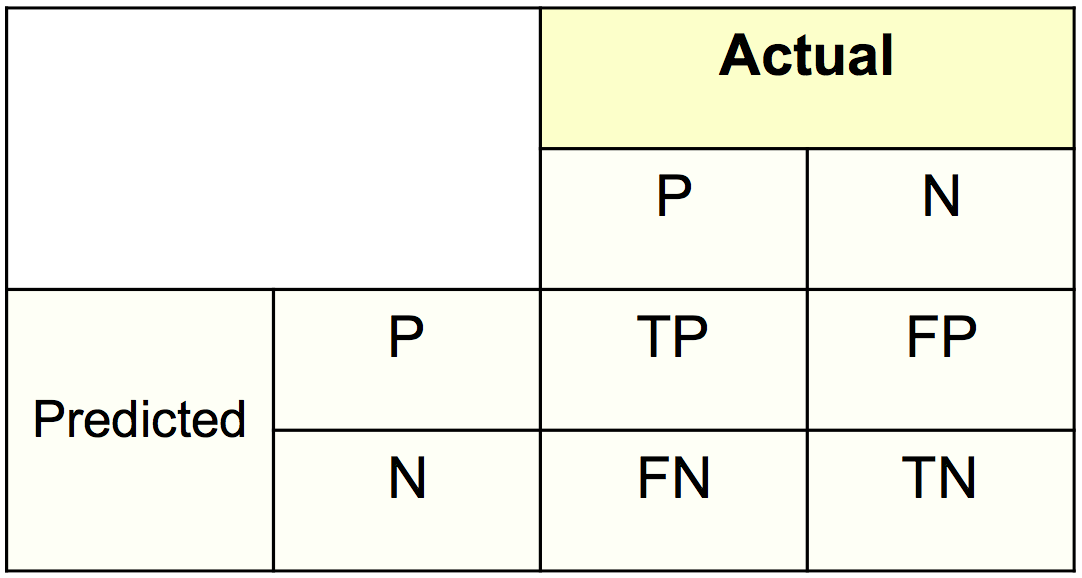
\includegraphics[width=0.3\textwidth]{img/img1}
	\caption{Possible prediction classification}
	\label{fig:1}
\end{figure}

\noindent\textbf{Precision} is the ratio of correctly predicted positive observations to the total predicted positive observations (Equation \ref{eq:1}). Specifically, the question that this metric answer is of all tweets that labeled as an emoji A, how many actually A? High precision relates to the low false positive rate.

\begin{equation}\label{eq:1}
Precision = \frac{TP}{TP + FP}
\end{equation}

\noindent\textbf{Recall} (Sensitivity) is the ratio of correctly predicted positive observations to the all observations in actual class (Equation \ref{eq:2}). Specifically, the question recall answers is: Of all the tweets that truly A, how many do we label?

\begin{equation}\label{eq:2}
Recall = \frac{TP}{TP + FN}
\end{equation}

\noindent\textbf{F1-score} is the weighted average of Precision and Recall. This score takes both false positives and false negatives into account. (Equation \ref{eq:3})

\begin{equation}\label{eq:3}
F1\textrm{-}score = \frac{2*Recall*Precision}{Recall + Precision}
\end{equation}


\section{Experiments \& Results}\label{lab:res}

We use two feature sets to evaluate the classifiers. The first feature set (\texttt{most100}) is a list of the 100 tokens which appear with the greatest frequency in the training set and the second feature set (\texttt{top10}) is the tokens whose presence was automatically determined to be predictive of one or more emoji classes. For each feature set, we employ Naive Bayes Algorithm and Decision Tree Algorithm separately. 

\subsection{Feature Analysis}
We evaluate the Naive Bayes Classifier using \texttt{top10} feature set. Table \ref{tab:1} shows the precision, recall,  and F1-score  of prediction on each emoji . We also added in the last column the occurrences of each emoji in the develop set.

From Table \ref{tab:1} we find that emoji \texttt{Disappoint} and \texttt{Facepalm} both get a low F1-score (0.253 and 0.175 separately), the reason may be there are few instances of these two emojis in the dataset and Naive Bayes usually has a poor performance on the class with few instances. 

\begin{table}
	\centering
	\begin{tabular}{c|ccc|c}
		\hline
		\textbf{Emoji} & \textbf{P} & \textbf{R} & \textbf{F} & \textbf{Num} \\
		\hline
		Clap &				0.206  &    \textbf{0.623}   & 0.309 & 1265 \\
		Cry & 				0.326    &  0.142   & 0.198 & 1587 \\
		Disappoint &  0.441    &  0.178   & 0.253 & 461 \\
		Explode & 		0.751    &  0.289   & \textbf{0.418} & 1334 \\
		FacePalm & 		0.410   &   0.111   & 0.175 & 433 \\
		Hands &			 0.696   &   0.249  &  0.367 & 1322 \\
		Neutral & 		0.165     & 0.444    &0.240 & 1496 \\
		Shrug & 		0.285    &  0.106   & 0.154 & 1222 \\
		Think  & 		\textbf{0.893}    &  0.053   & 0.100 & 1420 \\
		Upside & 		0.261    &  0.286  &  0.273& \textbf{1624} \\
		\hline
	\end{tabular}
	\caption{Precision, Recall, F1-score, and occurrences in the development set of the ten most frequent emojis using Naive Bayes + Pre.}
	\label{tab:1}
\end{table}

To evaluate the effectiveness of features. We choose some features which seem related to one or more particular emojis and delete these features. Because of the assumption that attributes are conditionally independent, delete some features would not influence other features. the comparison between predicted results on features with contain one and without it is meaningful, This experiment reveals the particular feature's influence on the classifier. For convenience, we use cross-validation with ten folders to build and evaluate the classifier. 

Table \ref{tab:2} shows the result of prediction on emoji \texttt{Explode} and \texttt{Think} with feature \texttt{army} and without it. The result shows that the feature \texttt{army} has great influence on the precision and recall of \texttt{Explode} (precision varies from 0.701 to 0.543 and recall varies from 0.297 to 0.317) and almost no influence on \texttt{Think} (almost no change in precision and recall). Which means that a sentence with word `army' tends to have higher or lower probability to use emoji \texttt{Explode},  but this word would have almost no help on the prediction of emoji \texttt{Think}. Therefore, choose high quality features is essential for a classification model.
\begin{table}[h]
	\centering
	\begin{tabular}{c|c|ccc}
		\hline
		\textbf{Emoji} & \textbf{Feature} & \textbf{P} & \textbf{R} & \textbf{F}  \\
		\hline
		\multirow{2}{*}{Explode} & $+\ army$ & 0.701   &   0.297   & 0.417 \\
		& $-\ army$ & 0.543    &  0.317   & 0.400 \\
		\hline
		\multirow{2}{*}{Think} & $+\ army$ & 0.055  &  0.104   &   0.204 \\
		& $-\ army$ & 0.055 &   0.104    &  0.205 \\
		\hline
	\end{tabular}
	\caption{Prediction on emoji \texttt{Explode, Think} with features contain \texttt{army} and removed it.}
	\label{tab:2}
\end{table}

\subsection{Algorithm Analysis}

To compare the performance of different classifier, we evaluate two classifiers on two feature sets. Table \ref{tab:4} shows the results of two classifiers on the two feature sets, first two rows are results on \texttt{most100}, next two rows are results on \texttt{top10}. From the table we find that for the same feature set, Naive Bayes always much faster than Decision Tree. Which is because Naive Bayes Classifier is very simple to build, extremely fast to make decisions, and easy to update the probabilities, it also scales easily for large number of dimensions (100s) and data sizes. 

\begin{table}[h]
	\centering
	\begin{tabular}{c|c|ccc|c}
		\hline
		\textbf{Fea} & \textbf{C} & \textbf{P} & \textbf{R} & \textbf{F} & \textbf{RT}\\
		\hline
		\multirow{2}{*}{most100} & NB & 0.330   &   0.304  &  0.303  &  0.73 \\
		& DT & 0.467  &    0.456   & \textbf{0.457}  & 127.7 \\
		\hline
		\multirow{2}{*}{top10} & NB &0.441  &    0.262  &  0.253  &  0.54 \\
		&	DT & 0.433   &   0.311  &  \textbf{0.302}  & 88.03  \\
		\hline
	\end{tabular}
	\caption{Results of two classifier Naive Bayes (NB) and Decision Tree (DT) on two feature sets. Evaluation on Precision (P), Recall (R), F1-score (F) and Run Time (RT).}
	\label{tab:4}
\end{table}

However, Naive Bayes Classifier has obvious disadvantages. The hypothesis that features are conditionally independent for a given class isn't always tenable and the model is too simple which makes it a general classifier but not custom-made for a particular task. In addition, this classifier is base on the probability which makes it perform bad on the labels with low frequency.

Compared with Naive Bayes Classifier, Decision Tree Classifier is time consumed but  achieve better performance on both precision and recall. As a machine learning algorithm, the  progress of constructing a tree is inexpensive. Simple construction and comparable performance make the algorithm very popular. However, it may fit a very complex tree structure to the data, which will leading to overfitting. Besides, it's accuracy depends a lot on the data presented. For example, the tree can become biased towards a specific class if it occurs a lot, or become "confused" when trying to fit certain rules inferred from the data. 

\begin{table}[h]
	\centering
	\begin{tabular}{c|cc|ccc}
		\hline
		\textbf{Fea} & \textbf{Leaves} & \textbf{Size} & \textbf{P} & \textbf{R} & \textbf{F}  \\
		\hline
		$+\ id$ & 1882 & 3763 & 0.346   &  0.292  &  0.284  \\
		$-\ id$ & 198 & 395 & 0.433  &   0.311  &  0.302   \\
		\hline
	\end{tabular}
	\caption{Decision Tree and its performance with add and remove feature \texttt{id}}.
	\label{tab:5}
\end{table}
	
To demonstrate the trait of Decision Tree classifier, we make a compare experiment between predictions with features include \texttt{id} and removed \texttt{id}. The experiment is build on cross-validation with ten folders. Table \ref{tab:5} shows the results. It shows that if we do not remove \texttt{id} from feature set, the constructed decision tree will extremely large (consist of 1882 leaves). The reason is that decision tree find a currently best feature as a decision point. So it has great probability to choose \texttt{id} as the root decision point because it can classify all instances base on this feature. In addition, we find the bad feature lead to a decrease of precision and recall of the classifier, precision is 0.433 without $id$ but only 0.346 with it. This phenomenon is a kind of overfitting.

\section{Conclusion}

In this report we compare the Naive Bayes and Decision Tree algorithm on a particular classification task. We find that Naive Bayes Classifier could get competitive result in a very short time and it scales easily for large number of dimensions and data size, which makes it the first choice for a new classification task. Whatever the classification is, we can build a Naive Bayes Classifier as baseline.

As for Decision Tree Classifier. It costs more time than Naive Bayes Classifier but also perform better than it on this task. It just builds a decision tree once and does not need to train which makes it one of the simplest model in machine learning area. The disadvantage is Decision Tree Classifier is easy to overfitting because of the elaborate divide of the instance.

In addition, good features can help classifier performance better. Generally, good features always have obvious bias distribution among different classes. For Naive Bayes Classifier, a bad features may have little helpful for classifier. However, for Decision Tree Classifier, bad features may have huge influence on the performance, eg:\texttt{id}. As a conclusion, in the future, we should try to find best features for our machine learning tasks.

\bibliographystyle{acl}
\bibliography{bibliography}

\end{document}
